\chapter{Revue de littérature}
\label{ch:litterature}

\section{Historique et concepts de la RA}
\label{sec:litterature_ar}

\cite{Sutherland1968} conçoit le premier visiocasque de RA \reffigureETSp{Sutherland1968.jpg} : ce prototype permet déjà de visualiser du contenu 3D affiché dans l'espace réel de l'utilisateur, donnant l'illusion que le contenu virtuel fait réellement partie de la pièce. Par la suite, la recherche académique en RA se développe lentement : les applications développées sont surtout à visées militaires et gouvernementales \citep{VanKrevelen2010}. Il faut alors attendre les années 1990, avec la miniaturisation des PCs, pour que le domaine de recherche s'établisse enfin. Plusieurs conférences dédiées à la RA sont notamment créées, fusionnées aujourd'hui sous le nom de International Symposium on Mixed and Augmented Reality (ISMAR), une conférence d'importance pour la recherche et l'industrie en RA \citep{Azuma2001}.

\figureETS[0.6]{Sutherland1968.jpg}{
  Photos du visiocasque de RA de Sutherland.\\
  Tiré de \cite{Sutherland1968}.
}

\cite{Milgram1994} donne un premier cadre théorique au domaine, en proposant une échelle ordonnée nommée \texten{Reality-Virtuality Continuum} \reffigureETSp{Milgram1994}. \citeauthor{Milgram1994} y oppose deux extrêmes : les environnements réels et les environnements virtuels. Les IHMs graphiques, en deux dimensions (2D), sur ordinateurs et téléphones font partie de la première catégorie, tandis qu'un visiocasque de RV, qui immerge totalement son utilisateur dans un monde virtuel en 3D, de la seconde. Entre ces deux extrêmes, les environnements de Réalité Mixte (RM), comme la RA, vont mélanger éléments réels et virtuels. La force de cette représentation est qu'il n'existe pas de catégories séparées entre réel, RA et RV mais que la RA peut se trouver d'un extrême à un autre le long de cette échelle.

Le second enseignement de l'échelle de \citeauthor{Milgram1994} est que RA et RV sont techniquement très proches : les dispositifs de localisation, d'affichage et de génération de contenu sont les mêmes \citep{Billinghurst2015}. Cependant, ces deux technologies n'ont pas les mêmes attentes. En effet, pour que l'immersion en RV fonctionne, il est nécessaire d'avoir un large champ de vision (\texten{field of view} ou FoV en anglais) ; par exemple, le champ de vision du visiocasque de RV HTC Vive est de \SI{100x113}{\degree} (horizontalement $\times$ verticalement) pour les deux yeux \citep{Kreylos2016}, ce qui est proche du champ de vision humain qui est de \SI{200x135}{\degree} pour les deux yeux \citep{ROMANIA_engineer2015}. La RA va en revanche demander tout d'abord une très grande précision et rapidité dans la localisation de l'utilisateur et des objets à augmenter pour donner le sentiment de « présence » du virtuel dans l'environnement réel.

\figureLayoutETS{Milgram1994}{%
  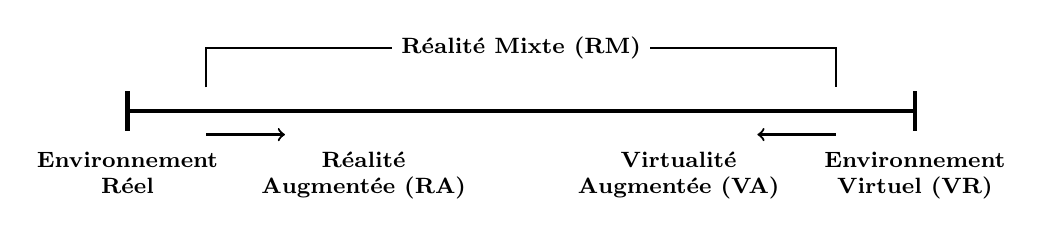
\begin{tikzpicture}[font=\footnotesize\bfseries]
    \tikzstyle{label}=[below, align=center, text depth=.25ex]
    
    \draw[ultra thick] (0,0) -- (10,0);
    \draw[ultra thick] (0,-0.25) -- (0,0.25);
    \draw[ultra thick] (10,-0.25) -- (10,0.25);

    \draw[thick, ->] (1,-0.3) -- (2,-0.3);
    \draw[thick, <-] (8,-0.3) -- (9,-0.3);

    \draw (0,-0.4) node[label] {Environnement\\Réel};
    \draw (3,-0.4) node[label] {Réalité\\Augmentée (RA)};
    \draw (7,-0.4) node[label] {Virtualité\\Augmentée (VA)};
    \draw (10,-0.4) node[label] {Environnement\\Virtuel (VR)};

    \draw[thick] (1,0.3) -- (1,0.8) -- (9,0.8) -- (9,0.3);

    \draw (5,0.8) node[fill=white] {Réalité Mixte (RM)};
  \end{tikzpicture}%
}{
  L'échelle du \texten{Reality-Virtuality Continuum} de Milgram.\\
  Adapté de \cite{Milgram1994}.
}

\cite{Rekimoto1995} apportent un second cadre théorique à la RA \reffigureETSp{Rekimoto1995.png}. Ils montrent que les IHMs graphiques sont coupées des interactions avec l'environnement réel, tandis que la RV isole l'utilisateur dans des IHMs totalement virtuelles. Deux alternatives à ces extrêmes sont la RA et l'informatique ubiquitaire (en anglais: \texten{ubiquitous computing}) : cette dernière permet à l'utilisateur d'interagir avec des ordinateur intégrés dans l'environnement réel, par exemple avec téléphones intelligents et des objets connectés, tandis que la RA fusionne réel et virtuel en un seul environnement pour l'utilisateur. Ainsi, avec une IHM bien faite, la RA s'intègre naturellement à l'environnement réel et devient invisible à l'utilisation.

\figureETS[0.7]{Rekimoto1995.png}{
  Comparaison de quatre styles d'IHMs : (a) les IHMs graphiques, coupées de l'environnement réel, (b) les IHMs en VR, isolant l'utilisateur dans un environnement virtuel, (c) l'informatique ubiquitaire, faite d'ordinateurs faisant partie intégrante de l'environnement réel et (d) les IHMs en RA faisant interface entre l'utilisateur et l'environnement réel.\\
  Tiré de \cite{Rekimoto1995}.
}

Une première définition formelle de la RA est par la suite proposée par \cite{Azuma1997} dans le premier état de l'art du domaine. Ainsi, la RA :
\begin{enumerate}
  \item combine des éléments réels et virtuels ;
  \item est interactive en temps réel ;
  \item aligne les éléments virtuels avec les éléments réels.
\end{enumerate}
\medskip

Ce sont les trois conditions techniques à respecter en RA qui vont donner le \emph{sentiment de la présence du virtuel} dans l'environnement réel. Autrement dit, ces conditions vont permettre à notre cerveau de percevoir virtuel et réel comme un seul et même environnement. Cette définition a le mérite d'être assez générale pour s'appliquer tout autant à la RA visuelle, qu'au RA auditives ou haptiques.

\figureETS[0.7]{Bimber2005.jpg}{
  Les différents dispositifs d'affichages en RA.\\
  Tiré de \citet{Bimber2005}.
}

Enfin, \cite{Buxton1998} repris par \cite{Bimber2005} catégorisent les différents dispositifs d'affichage en RA \reffigureETSp{Bimber2005.jpg}. On retient essentiellement (nous excluons volontairement les projecteurs) :
\begin{itemize}
  \item Le \texten{cave automatic virtual environnement} (CAVE) : c'est un environnement immersif sous forme d'un cube de \SI{3}{\m} de côté, chaque face comportant un écran \reffigureETSp{CAVE.jpg}. Les capteurs portés par l'utilisateur permettent au CAVE de suivre son mouvement et ainsi recalculer son champ de vision en temps réel. C'est un dispositif coûteux et encombrant, mais très utile pour prototyper des concepts.
  \item Les affichages fixes : la RA est affichée à travers un écran fixé dans l'environnement \reffigureETSp{Lee2013.jpg}.
  \item Les appareils mobiles : identique à un affichage fixe mais l'écran est tenu en main, comme une \emph{fenêtre sur le contenu} en RA \reffigureETSp{MobileAR.jpg}. Ils sont populaires mais limités en taille et en puissance \citep{Huang2013}.
  \item Les \texten{head-mounted display} (HMD) ou visiocasques en français : ils sont portés sur la tête et projettent les images virtuelles directement aux yeux de l'utilisateur. Ils ont l'avantage de laisser les mains libres. On distingue deux technologies :
  \begin{itemize}
    \item Les visiocasques vidéo : des caméras placées devant le casque filment l'environnement de l'utilisateur, les images capturées sont ensuite combinées avec le contenu virtuel puis affichées sur un écran \reffigureETSp{Piumsomboon2014_5.jpg}. Ils sont abordables et relativement facile à construire, mais la qualité de l'image est souvent faible \citep{Steptoe2013, Piumsomboon2014}.
    \item Les visiocasques optiques : le contenu virtuel est projeté sur un écran transparent par un système de miroirs. Il sont difficiles à concevoir et proposent un petit champ de vision, mais une image de très bonne qualité. C'est l'approche la plus privilégiée par les visiocasques de l'industrie, comme le HoloLens ou le Meta 2.
  \end{itemize}
  \item Les lentilles : elles sont identiques aux visiocasques mais posées directement sur les yeux. Peu utilisées, elles sont encore au stade de prototype mais, une fois maîtrisées, elles pourront être le dispositif de RA idéal \citep{VanKrevelen2010}.
\end{itemize}
\medskip

\figureETS[0.6]{CAVE.jpg}{
  Un CAVE : un cube immersif d'écrans à taille humaine réagissant aux déplacement de l'utilisateur. Ici, l'utilisateur tape la main de son propre hologramme.\\
  Tiré de \cite{Kreylos2012}.
}

\figureETS{Lee2013.jpg}{
  Photographies de SpaceTop : l'utilisateur peut déplacer des fenêtres dans espace 3D à travers un écran transparent en RA.\\
  Tiré de \cite{Lee2013}.
}

\figureETS[0.5]{MobileAR.jpg}{
  Une application sur tablette affichant un tableau de musée en RA.\\
  Tiré de \cite{Kippelboy2012}.
}

\figureETS[0.5]{Piumsomboon2014_5.jpg}{
  Photographie de l'AR-Rift, un visiocasque de RA vidéo dont la conception est documentée par \cite{Steptoe2013} : les images filmées par deux caméras sont retransmises dans un visiocasque de RV. \\
  Adapté de \cite{Piumsomboon2014}.
}

Tout ces dispositifs ont été explorés dans la littérature, mais ce sont essentiellement des prototypes sur appareils mobiles qui ont été développés : en effet, à partir des années 2000, les téléphones intelligents ont eu des caméras intégrées d'une qualité suffisante, tous les capteurs nécessaire et assez de puissance de calcul pour rendre la RA possible \citep{Huang2013}. Cependant, avec l'arrivée du HoloLens en 2016 les visiocasques vont pouvoir être à leur tour plus utilisés dans des recherches en RA.

Dans leur état de l'art \cite{Azuma2001} identifient les trois obstacles à dépasser pour que la RA puisse être utilisable par le grand public : (1) les limites techniques, (2) les limites des IHMs et (3) les problème d'acception sociale. Cependant, si quelques concepts et cadres théoriques pour la RA existent depuis plusieurs années, la recherche s'est malgré tout majoritairement consacrée à dépasser les limites techniques de la RA, comme le souligne \cite{Zhou2008}, \cite{VanKrevelen2010} et \cite{Billinghurst2015}, dans leurs états de l'art respectifs. Ils indiquent également que trop peu de travaux ont été consacrés aux IHM et à l'expérience utilisateur en RA : \textquote{\texten{there is a need to develop interface metaphors and interaction techniques specific to [augmented reality]
}} \citep{Billinghurst2015}.


\section{Conception et évaluation d'IHMs de RA}
\label{sec:litterature_ar_hci}

\subsection{IHMs en RA}
\label{subsec:litterature_ar_hci_presentation}

\figureLayoutETS{Billinghurst2005}{%
  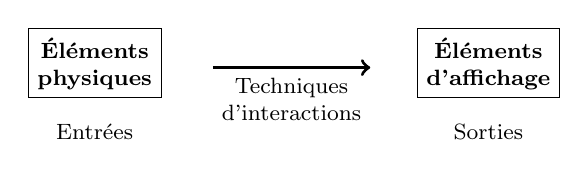
\begin{tikzpicture}[font=\footnotesize]
    \tikzstyle{label}=[below, align=center, text depth=.25ex]
    
    \draw (0,0) node[label, draw]{\textbf{Éléments}\\\textbf{physiques}};
    \draw (5,0) node[label, draw]{\textbf{Éléments}\\\textbf{d'affichage}};

    \draw[->, very thick] (1.5,-0.5) -- (3.5,-0.5)
      node[label, pos=0.5, below]{Techniques \\d'interactions};

    \draw (0,-1.1) node[label]{Entrées};
    \draw (5,-1.1) node[label]{Sorties};
  \end{tikzpicture}%
}{
  Principe d'une IHM : une technique interaction lie des entrées utilisateur, via un capteur physique, à un résultat affiché sur l'ordinateur.\\
  Adapté de \cite{Billinghurst2005}.
}

Une IHM constitue la principale interface avec laquelle un utilisateur va interagir avec un ordinateur. La bonne conception de cet intermédiaire est donc nécessaire pour rendre accessible et efficace le travail sur une machine. Son rôle est simple : comme le montre la \reffigureETS{Billinghurst2005}, il s'agit de lier des \emph{entrées utilisateurs} issues de capteurs physiques (souris, écran tactile, images d'une caméra) à des actions sur l'ordinateur représentées par un \emph{résultat en sortie} (affichage, son, commande) via une \emph{technique d'interaction} \citep{Billinghurst2005}. La technique d'interaction est donc \emph{une} méthode qui permet de traduire ces entrées en commandes : par exemple, le même mouvement avec une souris peut déplacer un curseur ou translater un objet le long d'un axe, ou encore un même déplacement de deux doigts sur un écran tactile peut faire une rotation ou un zoom sur un objet. Elle est également une métaphore qui permet à l'utilisateur d'associer ses actions avec des résultats sur l'ordinateur. Il existe de nombreux dispositifs d'entrée, de sortie et de techniques d'interaction, le défi étant de : \textquote{\texten{combine these together in a way that is most appropriate to the desired task, facilitates ease of use and learning and provides a high level of user performance and satisfaction}} \citep{Billinghurst2005}.

Un des but de la recherche en IHM est de réduire cet écart entre les éléments physiques et d'affichages \cite{VanDam1997}. \cite{Jacob2008} rappellent que les IHMs ont traversé plusieurs générations visant à chaque fois une utilisation plus simple, plus directe et plus proche des actions quotidiennes. Les ordinateurs s'utilisaient, avant les années 1960, par des cartes de commandes qui imprimaient alors leurs résultats. Puis ils ont été utilisés par ligne de commande via des terminaux jusque dans les années 1980. Enfin, les IHMs graphiques se sont démocratisées \reffigureETSp{Jacob2008.jpg}, suivants le paradigme WIMP : un ensemble de fenêtres (\texten{windows}), d'icônes (\texten{icons}) et de menus (\texten{menus}) accessibles par un appareil de pointage (\texten{pointing device}), comme une souris. Ces IHMs sont excellentes pour des applications graphiques en 2D, mais limitées pour celles en 3D, entre autres\footnote{Les IHMs en ligne de commande sont toujours utilisées et complémentaires des IHMs graphiques : elles peuvent être plus puissantes et mieux adaptées que ces dernières, même si elles sont plus difficile d'accès par le temps d'apprentissage qu'elles demandent.}. \cite{VanDam1997} appela alors à développer une nouvelle génération d'IHMs post-WIMP, c'est-à-dire contenant des techniques d'interactions non dépendantes de fenêtre, icônes ou de menu en 2D. L'objectif étant de diversifier les types d'IHMs pour proposer le plus adapté selon les besoins de l'utilisateur.

\figureETS[0.5]{Jacob2008.jpg}{
  Illustrations des deuxième (en ligne de commande) et troisième (par interface graphique WIMP) générations d'IHMs, ainsi que les nombreux types émergeants d'IHMs post-WIMP. Toutes sont complémentaires, chacune adaptée à des usages spécifiques qu'étudie la recherche sur les IHMs.\\
  Tiré de \cite{Jacob2008}.
}

Si de nombreuses IHMs post-WIMP ont par la suite été développées, comme celles désormais bien connues des téléphones intelligents à écrans tactiles \citep{Jacob2008}, aucun paradigme n'est encore établi pour la RA \citep{VanKrevelen2010}. \cite{Billinghurst2015} classent celles de RA en plusieurs catégories :
\begin{itemize}
  \item Navigateurs d'informations : affichant de l'information en RA sur l'environnement réel. Ce sont principalement les IHMs que l'on retrouve dans les applications pour téléphones intelligents \reffigureETSp{MobileAR.jpg} : elles permettent simplement d'afficher du contenu en surimpression de l'environnement réel, l'utilisateur se déplaçant simplement pour le voir sous différents angles. Des IHMs WIMP sont souvent utilisées, mais ce type d'interfaces est limité dans les interactions avec le contenu virtuel en 3D.
  \item Interfaces en 3D : utilisant des techniques d'interactions en 3D pour manipuler le contenu dans l'espace.
  \item Interfaces tangibles : utilisant des objets réels pour interagir avec du contenu virtuel.
  \item Interfaces naturelles : utilisant les mouvements du corps de l'utilisateur, par exemple des commandes gestuelles.
  \item Interfaces multimodales : utilisant simultanément des commandes vocales et gestuelles.
\end{itemize}
\medskip

Pour \cite{Billinghurst2015}, toutes ces IHMs importent et appliquent des techniques d'interactions des IHMs WIMP, de la RV ou utilisées avec des écrans tactiles. En ce sens, elles atteignent seulement les première et deuxième étapes du processus de \cite{Billinghurst2005} qui décrit les étapes de développement d'un paradigme d'IHM pour un nouveau média :
\begin{enumerate}
  \item développement de prototypes ;
  \item adoption de techniques d'interactions d'autres types d'IHM ;
  \item développement de métaphores et paradigmes d'IHMs adaptés au média ;
  \item développement de modèles théoriques pour ces paradigmes.
\end{enumerate}
\medskip

Pourtant, la RA présente un excellent média car l'écart entre les éléments physiques et d'affichage (le contenu virtuel) y est très réduit. Cela permettrait de fondre la présence de l'ordinateur dans l'environnement de l'utilisateur sans le restreindre sur un écran. Une bonne IHM de RA permettrait alors de manipuler naturellement et efficacement du contenu virtuel en 3D avec des techniques d'interactions basées sur des objets physiques, des commandes vocales ou des gestes utilisés au quotidien \citep{Billinghurst2005}. C'est pourquoi il est important de consacrer un effort de recherche pour atteindre cette troisième étape, comme nous souhaitons le faire avec notre concept de téléphone à écran étendu, en utilisant des IHMs en 3D, les IHMs naturelles et les IUTs. Enfin, on remarque que la classification des IHMs de RA de \cite{Billinghurst2015} se concentre quasi exclusivement sur les techniques d'interactions. Pourtant, les données affichées ont toute leur importance, et il s'agit également de dépasser les concepts de fenêtre, menu et icônes des IHMs WIMP.

\subsection{IHMs en 3D et IHMs naturelles}
\label{subsec:litterature_ar_hci_interactions}
Les IHMs en 3D sont importées des recherches de la RV et dans les environnements virtuels (EV) en 3D. La recherche sur les EVs explore les interfaces et les interactions avec du contenu en 3D affiché sur un écran (et non de manière immersive comme en RA). \cite{Bowman2004} classent les techniques d'interactions en trois catégories : (1) navigation, (2) sélection (un ou plusieurs objets) et (3) manipulation (translation et rotation). Seules ces deux dernières sont applicables à la RA, le contenu virtuel étant aligné et intégré avec l'environnement réel, l'utilisateur se déplace simplement lui-même pour y naviguer.

De nombreux dispositifs d'entrée ont été développés pour les IHMs en 3D : des souris 3D, des joysticks, des stylos suivis en 3D ou des dispositifs haptiques (avec retour de force, donnant l'illusion de toucher le contenu virtuel). Tous permettent de sélectionner et manipuler avec précision du contenu virtuel ; on parle alors de degrés de libertés (\texten{degrees of freedom} ou DoF en anglais) pour caractériser les manipulations possibles, avec un degré par dimension donc maximum trois pour la translation et trois pour la rotation : une souris standard permet donc 2 DoFs, quand les dispositifs d'entrées des visiocasques de RV sont suivis avec 6 DoFs \reffigureETSp{Evan-Amos2017.jpg}. Cependant, tous ces dispositifs présentent l'inconvénient d'occuper les mains de l'utilisateur : en RA, les espaces de visualisation et d'interaction sont donc séparés \reffigureETSp{Adcock2003.jpg} et les techniques d'interactions avec les objets virtuels sont alors différentes de celles avec les objets réels \cite{Billinghurst2015}.

\figureLayoutETS{3DControllers}{%
  \subfigureETS[0.2]{Evan-Amos2017.jpg}{Les dispositifs d'entrée du visiocasque de RV Oculus Rift : sans fils, ils permettent de sélectionner du contenu virtuel et de le manipuler avec 6 DoFs.}%
  \figurehspace%
  \subfigureETS[0.2]{Adcock2003.jpg}{IHM de RA où la main gauche utilise plusieurs boutons pour interagir avec le menu 2D, tandis que la main droite tient un stylo haptique pour manipuler le crâne en 3D.}%
}{
  Exemples de dispositifs d'entrées pour IHMS en 3D.\\
  Tiré de a) \cite{Evan-Amos2017} et b) \cite{Adcock2003}.
}

Les IHMs naturelles utilisent quant à elle directement les mouvements du corps de l'utilisateur comme dispositif d'entrée, en particulier les mains. De nombreuses méthodes de vision par ordinateur permettent ce suivi en utilisant simplement les images d'une caméra \citep{Billinghurst2015}. Un utilisateur peut alors en théorie agir directement avec du contenu virtuel comme il le ferait avec des objets réels. Malgré tout, de telles interactions demandent souvent des mouvements complexes et fatigants à l'utilisateur \citep{Bowman2001}. De plus, ces IHMs ne peuvent répliquer exactement de monde réel : le manque de contraintes physiques rends les interactions imprécises \citep{Chan2010} et il peut être difficile de comprendre comment interagir avec un environnement virtuel utilisant une IHM naturelle \citep{Argelaguet2013}.

\figureLayoutETS{NaturalControllers}{%
  \subfigureETS[0.2]{Taylor2016.jpg}{Main virtuelle.}%
  \figurehspace%
  \subfigureETS[0.2]{Argelaguet2013.jpg}{Pointeur virtuel.}%
}{
  Deux techniques d'interactions de sélection dans les IHMs naturelles.\\
  Tiré de a) \cite{Taylor2016} et b) \cite{Argelaguet2013}.
}

Un écart existant donc toujours entre éléments physiques et éléments graphiques, des techniques d'interactions sont toujours nécessaires ; deux types de techniques sont majoritairement utilisées. La \emph{main virtuelle} affiche un modèle 3D de main pouvant interagir avec le contenu virtuel et suivant la main réelle de l'utilisateur \reffigureETSp{Taylor2016.jpg}. Elle est la plus naturelle, mais souffre particulièrement des problématiques que nous venons d'énoncer, mais aussi de problème d'occlusion, car elle peut cacher des objets virtuels. La technique du \emph{pointeur virtuel} permet à l'inverse de projeter un rayon, depuis la main ou la tête, pour sélectionner des objets \reffigureETSp{Argelaguet2013.jpg} : il permet de facilement atteindre des objets lointains avec peu d'effort, mais cela est difficile s'ils sont de trop petite taille. De plus, si l'action de sélection peut entraîner un déplacement involontaire du pointeur, par exemple en pressant un bouton \citep{Argelaguet2013}. Cette technique a notamment été choisie pour le HoloLens : le pointeur suit les mouvements de la tête, stables et précis \citep{Kitoe2018}, tandis que la sélection se fait avec un geste de la main pour ne pas perturber le pointage.

La difficulté pour ce type d'IHM est donc de permettre des sélections et manipulations rapides, sans erreurs ainsi que d'être faciles à comprendre et peu fatigantes \citep{Argelaguet2013}. Pour cela, il est crucial de fournir des retours à l'utilisateur : \cite{Chan2010} propose la combinaison de retours continus, pour que l'utilisateur situe le suivi de son corps, et de retours discret pour confirmer ses ses actions. Le modèle 3D de la main virtuelle avec des ombres portées ou le rayon du pointeur virtuel sont donc des retours visuels continus, tandis qu'un bref changement de couleur de l'objet peut confirmer une sélection. Ces retours ne doivent cependant pas être excessifs, au risque de produire une distraction et réduire la performance des utilisateurs \citep{Argelaguet2013}.

\figureETS[1]{Piumsomboon2013_1.jpg}{
  Les onze poses de mains utilisées pour des gestes en RA.\\
  Tiré de \cite{Piumsomboon2013}.
}

\figureETS[1]{Piumsomboon2013_2.jpg}{
  Extrait de la liste de gestes pour différentes tâches en RA. Les positions de mains utilisables sont indiquées entre crochets.\\
  Tiré de \cite{Piumsomboon2013}.
}

Si l'utilisation du pointeur virtuel par le HoloLens fait actuellement consensus \citep{Kitoe2018}, ce n'est pas le cas pour la main virtuelle dans les IHMs de RA malgré de nombreux prototypes \citep{Piumsomboon2013}. \citeauthor{Piumsomboon2013} ont alors établi de manière rigoureuse une liste de gestes utilisables avec une main virtuelle en RA. Pour cela, ils ont tout d'abord montré des animations de quarante tâches courantes dans la littérature dans un visiocasque de RA à vingt participants et leur ont demandé de mimer en même temps que chaque animation le geste qu'ils utiliseraient. Ils ont alors sélectionné les \emph{poses} de main les plus utilisées \reffigureETSp{Piumsomboon2013_1.jpg}, ainsi que le ou les \emph{gestes} majoritaires avec un score de consensus pour chaque tâche \reffigureETSp{Piumsomboon2013_2.jpg}. Beaucoup de tâches ont un faible consensus (peu de participants ont utilisé le même geste), néanmoins ceux pour les menus ont un haut score $\geq 80\%$ \reffigureETSp{Piumsomboon2013_3.jpg}. Enfin, on remarque que la majorité de ces gestes sont réalisés \textquote{en l'air}, à l'exception de ceux ouvrant, fermant et sélectionnant un menu horizontal qui ont été réalisés sur la surface de la table \reffigureETSp{Piumsomboon2013_2.jpg}.

\figureETS[0.9]{Piumsomboon2013_3.jpg}{
  Score de consensus sur le geste à utiliser (barres bleues) ainsi que ratio de gestes à deux mains (ligne rouge) parmi les participants pour chaque tâche.\\
  Tiré de \cite{Piumsomboon2013}.
}

Par la suite, \cite{Piumsomboon2014} ont comparé formellement quelques-unes de ces techniques avec des commandes vocales pour la sélection et la manipulation d'objets en 3D dans un visiocasque de RA. Leurs résultats indiquent que les participants étaient globalement plus rapides et préféraient utiliser des gestes pour manipuler les objets, mais des commandes vocales pour les redimensionner. Il serait cependant intéressant de reproduire cette étude avec des IHMs plus complexes que de simples objets 3D, par exemple avec des IHMs WIMP appliquées à la RA, comme le fait le HoloLens.

\figureLayoutETS{Piumsomboon2014_1}{%
  \subfigureETS[0.17]{Piumsomboon2014_1.jpg}{La main virtuelle fait occlusion avec le contenu 3D.}%
  \figurehspace%
  \subfigureETS[0.17]{Piumsomboon2014_2.jpg}{Le contenu 3D est transparent, laissant visible la main de l'utilisateur.}%
}{
  Différentes techniques d'occlusion de la main.\\
  Tiré de \cite{Piumsomboon2014}.
}

Enfin, \cite{Piumsomboon2013} et \cite{Piumsomboon2014} recommandent, à la suite d'études pilotes, que pour éviter les problèmes d'occlusion, les objets virtuels doivent toujours êtres visibles : soit en utilisant une main virtuelle transparente plutôt qu'opaque, soit en affichant leurs contours si elle les cache \reffigureETSp{Piumsomboon2014_1}.

citer études avec mains virtuelles : \cite{Chan2010}, \cite{Markussen2014} et \cite{Hincapie-Ramos2014}

\subsection{IHMs de RA tangibles}
\label{subsec:litterature_ar_hci_tui}
Les IHMs de RA tangibles utilisent des objets réels comme dispositifs d'entrées et d'affichages, qui sont alors augmentés par RA \citep{Kato2000}. Autrement dit, chaque objet virtuel est aligné avec un objet réel et est manipulé via cet objet réel \citep{Billinghurst2005} : les espaces d'interactions et d'affichage sont donc alignés \citep[p. 170]{Billinghurst2015}. Ainsi, les interactions sont familières, faciles et intuitives et peuvent s'appuyer sur les contraintes physiques de ces objets réels \citep{Zhou2008}. Le principal inconvénient de ces IHM est de requérir des objets physiques, qui peuvent ne pas être présents dans l'environnement de l'utilisateur ou difficiles à transporter dans un usage mobile.

\figureLayoutETS{Lee2004}{%
  \subfigureETS[0.25]{Lee2004_1.jpg}{L'utilisateur presse les boutons du navigateur, puis créé l'objet courant en le pointant avec le cube de manipulation.}%
  \figurehspace%
  \subfigureETS[0.25]{Lee2004_2.jpg}{L'utilisateur déplace l'objet crée avec le cube, puis le fixe en cachant le haut du cube. Il le place dans la corbeille pour le détruire.}%
  \figurehspace%
  \subfigureETS[0.25]{Lee2004_3.jpg}{Redimensionnement d'un cube à l'aide d'un clavier connecté à un outil inspecteur affichant la propriété de taille du cube.}%
}{
  Exemple d'une IHM de RA tangible : les objets virtuels sont alignés avec des objets réels suivis avec 6 DoF et manipulés via des objets virtuels spécifiques utilisés comme outils.\\
  Tiré de \cite{Lee2004}.
}

Il existe encore un écart entre entrées et affichages pour ce type d'IHM, en particulier pour certaines commandes : par exemple, pour changer les dimensions de l'objet virtuel ou, de manière générale, ses propriétés, l'activer ou encore réaliser des opérations de copie. Des techniques d'interactions sont donc toujours nécessaires, la difficulté étant de faire comprendre l'utilisateur les commandes possibles et les conséquences de ces actions \citep{Zhou2008}. \cite{Lee2004} proposent par exemple d'utiliser certains objets réels comme des outils pour créer, détruire les autres objets virtuels ainsi que visualiser et modifier leurs propriétés : l'utilisateur place les outils proches des objets pour les faires interagir puis passe son doigt dessus comme pour effectuer un clic pour les activer \reffigureETSp{Lee2004}.

Il existe deux approches pour concevoir une IHM de RA tangible : une seule fonction est attribuée à chaque outil dans une IHM à \emph{multiplexage spatial}, tandis qu'un même outil est utilisé pour plusieurs fonctions selon le contexte dans une IHM à \emph{multiplexage temporel} \cite[p. 171]{Billinghurst2015}. Le multiplexage spatial est plus facile à apprendre, mais le multiplexage temporel permet plus de flexibilité dans la conception de l'IHM. Par exemple, le cube de manipulation dans l'IHM de \cite{Lee2004} est à multiplexage spatial (il a une seule fonction), tandis que l'outil inspecteur est à multiplexage temporel, car il affiche des données différentes en fonction de l'objet et de la propriété inspectés.

\figureLayoutETS{Lee2011}{%
  \subfigureETS[0.15]{Lee2011_1.jpg}{Navigateur d'information : le menu apparaît à distance fixe de l'utilisateur.}%
  \figurehspace%
  \subfigureETS[0.15]{Lee2011_2.jpg}{Tangible et aligné avec l'écran d'un téléphone tenu en main.}%
  \figurehspace%
  \subfigureETS[0.15]{Lee2011_3.jpg}{Tangible et aligné avec un objet de l'environnement.}%
}{
  Affichage d'un même menu selon différents types d'IHM de RA.\\
  Tiré de \cite{Lee2011}.
}

\figureLayoutETS{White2009}{%
  \parbox{0.965\textwidth}{% Allow line breaks
    \centering%
    \subfigureETS[0.15]{White2009_1.jpg}{Quand le menu est activé, il est aligné avec un objet tenu en main.}%
    \figurehspace%
    \subfigureETS[0.15]{White2009_2.jpg}{Le menu peut alors rester tenu en main.}%
    \figurehspace%
    \subfigureETS[0.15]{White2009_3.jpg}{Le menu peut rester attaché à la tête de l'utilisateur.}%
    \\%
    \subfigureETS[0.15]{White2009_4.jpg}{Le menu peut rester fixe dans l'espace.}%
    \figurehspace%
    \subfigureETS[0.15]{White2009_5.jpg}{Le menu peut être attaché à une planche : la sélection est alors bi-manuelle.}%
    \figurehspace%
    \subfigureETS[0.15]{White2009_6.jpg}{La sélection d'un élément du menu se fait en le pointant avec l'objet tenu en main.}%
  }%
}{
  Différents placements possibles d'un menu de RA.\\
  Tiré de \cite{White2009}.
}

Un téléphone peut donc être utilisé comme base d'IHM de RA tangible, par exemple pour afficher des menus alignés avec l'écran \reffigureETSp{Lee2011}. \cite{White2009} ont comparé l'usage un tel menu aligné avec d'autres placements possibles, par rapport à la tête de l'utilisateur ou par rapport à l'environnement \reffigureETSp{White2009}. L'utilisateur sélectionne un élément du menu en le pointant avec l'objet tenu en main. Dans les résultats de leur étude expérimentale, où treize participants ont effectué chacun 80 sélections avec chaque type de menu, leurs résultats indiquent que les sélections ont été statistiquement plus rapides dans les cas du menu tenu en main ou attaché à la tête de l'utilisateur (en moyenne en \SI{3}{\s} contre \SIrange{7}{8}{\s}). Les utilisateurs ont également préféré ces deux techniques. Pour \citeauthor{White2009} ces deux conditions étaient les plus stables et les plus faciles à utiliser. Pourtant le menu attaché à la main est plus intéressant car l'utilisateur peut facilement le déplacer ou changer son orientation. Cette étude supporte donc la faisabilité d'une IHM de RA tangible basée sur un téléphone tenu en main.

\subsection{Évaluation d'IHM en RA}
\label{subsec:litterature_ar_hci_evaluation}
Pour déterminer si une IHM est fonctionnelle et pertinente, il convient de l'évaluer dans des études utilisateurs \cite[p. 189]{Billinghurst2015}. En outre, cela permet de donner des clés de conception à d'autres chercheurs dans le domaine.

\cite{Swan2005} et \cite{Duenser2008} catégorisent les études utilisateurs en RA selon les questions qu'elles visent : (1) perception et cognition humaine en RA, (2) interactions en RA et (3) communication et collaboration en RA. Seule une minorité des articles contenaient alors une étude utilisateur (environ 10\%), la plus grande part d'entre elles étant consacrée à aux d'interactions (et IHMs).

Il existe plusieurs méthodes :
(1) Objective measurements : performance (temps, erreurs, efficacité), surtout temps de complétion et taux d'erreur, ou encore score, position, nombre d'actions, mouvements\\
(2) Subjective measurements : engagament, retour utilisateur, questionnaires, notes utilisateurs, retours utilisateurs\\
(3) Qualitative analysis : avis d'experts, observations, interviews formelles, classification des comportements utilisateurs\\
(4) Usability evaluation techniques : évaluations experts, évaluations heuristiques, analyse de tache, description à haute voix, méthode magicien d'Oz\\
(5) Informal evaluations : observations utilisateurs, retours utilisateurs

Swan2005, Duenser2008 (p.203) : evaluation en RA

\cite[p. 20]{Jankowski2015}

taches plus écologiques (proches des usages réels du quotidien)

Une fois les mesures faites, il convient de les analyser pour en tirer un sens notamment à l'aide d'outils statistiques. En pratique, on cherche souvent à montrer des différences, par exemple entre deux techniques pour montrer que l'une est meilleure que l'autre. On dit qu'une des techniques a un effet sur la performance (temps, erreurs) par rapport à l'autre. Or, on n'a pris des mesures que sur un \emph{échantillon} de la \emph{population}, qu'on espère suffisamment représentatif, lors des études utilisateurs. On peut analyser les mesures de l'échantillon, mais on souhaiterait pouvoir dire si cela est également applicable à la population.

Le test de l'hypothèse nulle est couramment utilisé pour cela dans la littérature en IHM. On postule une hypothèse alternative qu'on nomme l'hypothèse nulle : par exemple, les deux techniques n'ont pas d'effet sur la performance des utilisateurs. On calcule alors la probabilité, la \emph{valeur-p}, d'observer de tels résultats s'il n'y avait en réalité pas d'effet, si l'hypothèse nulle est vraie. Typiquement, on se donne 5\% de chance d'erreur, c'est-à-dire qu'on considère que si $p < 0.05$ alors on peut rejeter l'hypothèse nulle et dire qu'il y a un effet \emph{statistiquement significatif} : on considère que ce serait trop improbable d'obtenir de tels résultats s'il n'y avait pas d'effet. La valeur-p n'est cependant \emph{pas} la probabilité qu'il n'y ait pas d'effet.

Pourtant cette pratique est controversée. Premièrement, si on se donne une chance d'erreur sur chaque test, plus on effectuera de tests, plus on aura de chance d'avoir rejeté à tord l'hypothèse nulle : c'est le problème des comparaisons multiples. Par exemple, pour $20$ tests, on a probablement déclaré $20 \times 0.05 = 1$ effet significatif alors qu'il n'y a en réalité pas d'effet. En pratique, il est possible de réduire ce risque à l'aide des méthodes de correction. Deuxièmement, on ne sait pas la taille de l'effet en lui-même, s'il y en a un, ni on ne peut conclure quoi que ce soit si la valeur-p est trop élevée. \cite{Dragicevic2016} propose alors de remplacer les tests de l'hypothèse nulle avec le calcul d'\emph{intervalles de confiance} : c'est un intervalle qui indique les valeurs plausibles autour de la moyenne. Il mesure alors \emph{l'importance significative} de l'effet.

Dès lors, on peut considérer que la valeur-p et l'intervalle de confiance donnent en pratique la même information. Pourtant le test de l'hypothèse nulle reste couramment utilisé dans la littérature en IHM. C'est pourquoi nous avons choisis dans ce mémoire de les utiliser conjointement.
%The interval estimate indicates the uncertainty around the point estimate. The most common type of interval estimate is the confidence interval. It captures the population mean 95\% of the time across many replications. In practice, it is simpler to think of a confidence interval as a range of plausible values for the population mean. The point estimate is the most plausible, and plausibility smoothly decreases as we move away from it. Plausibility does not suddenly drop when crossing the limits, as values outside are implausible but not impossible.

%What the p-value captures is the probability of observing results as extreme as (or more extreme than) what was actually observed if the null hypothesis was true. In practice, it is easier to think of a p-value as a measure of strength of evidence against the null hypothesis; The closer p is to 0, the stronger the evidence that the null hypothesis is false. So p is computed under the assump tion that the null hypothesis is true. Yet it is common for researchers, teachers and even textbooks to think of p as the probability of the null hypothesis being true (or equivalently, of the results being due to chance).

%P-values capture what is traditionally termed statistical significance, while effect sizes capture practical significance (Kirk 2001).

%We cannot conclude anything from a high p-value, because it tells us that zero is plausible, but says nothing about other plausible values. Despite this, few researchers can resist the temptation to conclude that there is no effect. Plotting confidence intervals eliminates the problem.

%P is a function of the mean and the standard deviation (and sample size, if not held constant). Thus the p-value obtained would be different for the exact same reasons: sampling variability. Any statistical calculation is subject to sampling variability. This is also true for confidence intervals. By definition, only 95\% of these will capture the population mean in the long run.

%There rarely seems to be a good reason to report p-values in an HCI research paper, since confidence intervals can present the same information and much more, and in a much clearer, more usable manner. Perhaps the only remaining argument in favor of p-values is that they are useful for formally establishing statistical significance. But as we will now see, the notion of binary significance testing is a terrible idea for those who want to achieve fair statistical communication.

%Tips:
%Tip 12: Consider the log transform. The procedure consists in log-transforming all raw time measurements, performing all analyses as usual, then converting back (antilog ging) the means and confidence interval limits at the very end, when they need to be presented numerically or graphically. All means will indicate eometric (instead of arithmetic) means, and differences between means will become ratios.

%Tip 14: Do not test for normality. The world is not sharply divided into normal and non-normal distributions. When computing exact confidence intervals, departures from normality are not such a big deal. Measurement scales that are strictly positive (e.g., time) orbounded (e.g., percents) cannot be normally distributed. Strictly positive scales are typically positively skewed and approximate a normal distribution once logged (Tip 12).

%Tip 16: Prefer pictures. However, because the numerical format is more compact, it can be used for reporting secondary results, e.g. 2.9kg, 95\% CI [0.02, 5.8].

%Tip 26: Use vague language and hedges. We could say that Fig.13.6 “provides good evidence that B outperforms A, whereas C and A seem very similar, and results are largely inconclusive concerning the difference between D and A.” The use of vague language is necessary for acknowledging and honestly conveying the uncertainty present in effect size estimates.

%Tip 27 : Never say “no effect”. Almost any experimental manipulation has some effect on human behavior. Better wordings include “the direction of the effect is uncertain, but it is likely small”, or “we were not able to measure an effect”.


\section{Espaces de travail en RA}
\label{sec:litterature_ar_worspaces}
La séparation entre les styles d'IHMs présentées \cite{Rekimoto1995} \reffigureETSp{Rekimoto1995.png} est artificielle : comme nous l'avons vu, l'échelle de \cite{Milgram1994} nous montre que la RA devrait s'intégrer avec l'informatique ubiquitaire, les IHMs graphiques et la RV \cite{Billinghurst2005}. Par exemple, \cite{Heun2013} utilise la RA comme interface pour interagir de façon naturelle avec les objets intelligents autour de soi \reffigureETSp{Heun2016.jpg}, tandis que le prototype SpaceTop de \cite{Lee2013} permet de placer les fenêtres d'une IHM WIMP sur une grille en 3D \reffigureETSp{Lee2013.jpg}.

\figureETS[0.7]{Heun2016.jpg}{
  Photographie du \texten{Reality Editor}, un navigateur web de RA pour interagir facilement avec les objets intelligents autour de soi. Ici, une personne paye un parc-mètre via son téléphone.\\
  Tiré de \cite{Heun2016}.
}

Google Glass a été une expérience novatrice de visiocasque. Malgré les problèmes de vie privée et d'acceptation sociale que son usage a posé, \cite{Koelle2015} rappellent que cela a montré qu'il était intéressant de combiner un visiocasque de RA avec un téléphone intelligent : l'utilisateur interagissant avec son téléphone via le visiocasque, par des interactions multimodales à la voix ou encore avec des gestes en l'air décodés par la caméra du visiocasque. Cette expérience montre ainsi que les visiocasques de RA vont d'abord prendre place dans nos quotidiens professionnels où ils seront mieux acceptés ; c'est également la stratégie de la nouvelle version de ce visiocasque \cite{Levy2017}. Il est donc plus intéressant d'orienter des recherches en IHM pour la RA

Le Google Glass était un prototype limité visible seulement par l'\oe il droit avec un faible champ de vision \reffigureETSp{Phandroid2013_1.jpg}, mais surtout sans proposer une véritable IHM de RA : affichée sur un unique plan virtuel à une distance fixe des yeux de l'utilisateur \reffigureETSp{Phandroid2013_2.jpg}, comme sur la \reffigureETS{White2009_3.jpg}, elle ne répond pas à l'alignement virtuel-réel dans la définition d'\cite{Azuma1997}. Aussi, cette fenêtre virtuelle peut faire occlusion avec l'environnement réel, et gêner la vue de l'utilisateur. De nombreux autres visiocasques, comme Epson Moverio ou Vusix, souffrent de ces mêmes limites. C'est pourquoi le HoloLens a apporté une innovation majeure dans l'industrie de la RA en proposant de placer de multiples fenêtres virtuelles contre les mur, comme on peut accrocher un tableau, donnant réellement le sentiment qu'elles font partie de l'environnement réel.

\figureLayoutETS{Glass}{%
  \subfigureETS[0.2]{Phandroid2013_1.jpg}{Utilisateur portant le visiocasque : le champ de vision est très petit et limité à l'\oe il droit.}%
  \figurehspace%
  \subfigureETS[0.2]{Phandroid2013_2.jpg}{Vue depuis le visiocasque : l'IHM est affichée sur un rectangle à distance fixe de l'utilisateur sans intégration avec l'environnement réel.}%
}{
  Photographies du Google Glass.\\
  Tiré de \cite{Phandroid2013}.
}

Partant de la mêmes limite d'un seul écran de ces visiocasques, \cite{Ens2014} proposent alors le Personal Cockpit, une IHM de RA affichant de multiples fenêtres autour de l'utilisateur \reffigureETSp{Ens2014}. Il peut y organiser l'information sur différents écrans qui le suivent dans ces déplacements et avec qu'il interagit directement avec une technique de main virtuelle. \citeauthor{Ens2014} mesurent alors qu'un utilisateur travaille 40\% plus rapidement avec de multiples fenêtres qu'avec une simple fenêtre fixe en faisant du multi-tâches. Ils y évaluent également plusieurs facteurs de conception : leurs résultats indiquent (1) qu'un affichage courbe est moins fatiguant et moins sujet à des erreurs de sélection, les fenêtres étant ainsi affichées à la même distance de l'utilisateur, (2) que les interactions avec une main virtuelle sont plus stables et faciles avec des fenêtres fixées dans l'espace que placées sur le corps, car l'utilisateur peut les faire bouger involontairement et (3) la distance minimum des fenêtres est \SI{50}{\cm} de l'utilisateur, provoquant autrement de l'inconfort. Cependant, leur étude utilisait un CAVE simulant un petit champ de vision de $\ang{40} \times \ang{30}$ : il serait alors intéressant de la reproduire avec visiocasque à large champ de vision.

\figureLayoutETS{Ens2014}{%
  \subfigureETS[0.12]{Ens2014_1.jpg}{Positionnement idéal des fenêtres virtuelles en un affichage courbe.}%
  \figurehspace%
  \subfigureETS[0.12]{Ens2014_2.jpg}{Exemple d'utilisation avec une carte de navigation.}%
}{
  Photographies et illustrations du Personal Cockpit.\\
  Tiré de \cite{Ens2014}.
}

Avec MultiFi, \cite{Grubert2015} explorent de leur côté comment combiner les entrées et les sorties des appareils intelligents que nous portons (téléphone, tablettes, montre) avec un visiocasque de RA. Ces appareils mobiles ne sont souvent pas conçus pour travailler ensemble, mais gagneraient à l'être. La \reffigureETS{Grubert2015_2.jpg} montre par exemple une liste affichée sur une montre à l'écran étendu : en plaçant son téléphone sur un élément de la liste, l'utilisateur peut alors le voir en détails. Les différentes tailles et définitions d'affichage sont ainsi exploitées pour composer une seule vue pour l'utilisateur. \citeauthor{Grubert2015} distinguent alors trois alignements possibles entre une fenêtre virtuelle de RA et un appareil mobile \reffigureETSp{Grubert2015_1.jpg} :
\begin{enumerate}
  \item mode \texten{body-aligned} : la fenêtre a pour référence le corps de l'utilisateur, comme \cite{Ens2014}, l'appareil mobile formant alors une vue \texten{detail} sur le contenu (\reffigureETS{Grubert2015_3.jpg}, similaire à \cite{Berge2014}) ;
  \item mode \texten{device-aligned} : la fenêtre est centrée et alignée sur l'appareil mobile dont elle étend l'écran \reffigureETSp{Grubert2015_2.jpg} ;
  \item mode \texten{side-by-side} : un des appareils, visiocasque compris, redirige ces interactions vers un autre appareil, par exemple les interactions tactiles du téléphone vers une fenêtre virtuelle.
\end{enumerate}
\medskip

\figureETS{Grubert2015_1.jpg}{
  Illustrations des alignements possibles de contenu entre un visiocasque de RA et un appareil mobile : le mode \texten{body-aligned} à gauche, le mode \texten{device-aligned} au milieu et le mode \texten{side-by-side} à droite.\\
  Tiré de \cite{Grubert2015}.
}

Leurs résultats expérimentaux, dans une tâche de recherche d'information et de pointage, montrent que le couplage des appareils mobiles avec un visiocasque de RA peut permettre des temps plus rapides par rapport aux appareils seuls, visiocasque compris, mais au détriment d'un plus grand effort perçu par les utilisateurs. En outre, les préférences des utilisateurs étaient variées, ce qui montre que le choix du couplage entre appareils mobiles et visiocasque doit être laissé à l'utilisateur. Cependant, le visiocasque utilisé était lourd et avait aussi un petit champ de vision de $\ang{31} \times \ang{17}$ : ne pouvant pas voir de large contenu en une fois, les participants devaient fréquemment bouger la tête. De plus, seules des interactions sur les écrans tactiles, ou en plaçant l'appareil mobile dans l'espace, ont été évaluées. Il serait intéressant de les comparer avec des interactions utilisant une main virtuelle, et dans un visiocasque avec un large champ de vision.

\figureLayoutETS{Grubert2015_Demos}{%
  \subfigureETS{Grubert2015_2.jpg}{Une montre intelligente à écran étendu par RA en haut (mode \texten{device-aligned}). En bas, un téléphone intelligent placé sur la fenêtre virtuelle permet de la voir de manière plus détaillé : c'est une vue \texten{detail} sur l'écran étendu qui est alors une vue \texten{overview}.}%
  \figurehspace%
  \subfigureETS{Grubert2015_3.jpg}{L'utilisateur pointe son téléphone vers des éléments affichés par le visiocasque en mode \texten{body-aligned} pour les voir en détail.}%
}{
  Photographies de MultiFi.\\
  Tiré de \cite{Grubert2015}.
}

\cite{Serrano2015} généralisent avec Gluey le mode \texten{side-by-side} de MultiFi. Un visiocasque de RA affichant du contenu virtuel en permanence sans encombrer les mains de son utilisateur est le support idéal pour transmettre de l'information facilement entre différents appareils. Par exemple, une personne peut utiliser un clavier, une souris ou un écran tactile et voir ses actions s'exécuter sur un autre appareil qu'il regarde \reffigureETSp{Serrano2015_1.jpg}, ou encore copier des données depuis un ordinateur et les \textquote{coller} sur une imprimante pour les imprimer \reffigureETSp{Serrano2015_Demos}. Pour \citeauthor{Serrano2015}, les fonctionnalités d'une telle IHM sont (1) la redirection des entrées entre les appareils, (2) la migration du contenu entre les appareils, (3) la compatibilité de tous les appareils pour 1 et 2, (4) l'identification des appareils disponibles, (5) l'identification de leurs positions, (6) donner des retours de ces actions à l'utilisateur et (7) être mobile. Ainsi, MultiFi ne satisfait qu'aux critères 1, 5, 6 et 7. L'article de \citeauthor{Serrano2015} présente toutefois des limites, par la faiblesse de son évaluation, informelle, qui a seulement montré que le prototype de leur était, mais aussi par le faible champ de vision de leur visiocasque.

\figureETS[1]{Serrano2015_1.jpg}{
  Illustration du concept de Gluey : le visiocasque de RA sert de support intermédiaire pour transmettre de l'information facilement entre tous les appareils disponibles.\\
  Tiré de \cite{Serrano2015}.
}

\figureLayoutETS{Serrano2015_Demos}{%
  \subfigureETS[0.3]{Serrano2015_2.jpg}{Copie du lien d'une vidéo vers le presse-papier du visiocasque.}%
  \figurehspace[2]%
  \subfigureETS[0.3]{Serrano2015_3.jpg}{Impression d'une image en la déplaçant du presse-papier du visiocasque pour la déposer sur l'imprimante.}%
}{
  Photographies du fonctionnement de Gluey.\\
  Adapté de \cite{Serrano2015}.
}

Enfin, \cite{Serrano2015a} ont complété Gluey en proposant un concept de \emph{bureau virtuel} qu'ils ont nommé Desktop-Gluey. Cette série d'IHMs permet d'intégrer des fenêtres virtuelles dans un environnement de travail de bureau. Leur première idée est de les utiliser en parallèle d'écrans d'ordinateur voire de les remplacer tout en continuant à utiliser clavier et souris, comme avec Gluey \reffigureETSp{Serrano2015a_1.jpg}. Ces fenêtres virtuelles peuvent également être placées pour étendre les écrans physique comme dans le mode \texten{device-aligned} de MultiFi ou dans des dispositions spatiales similaires au Personal Cockpit \reffigureETSp{Serrano2015a_2.jpg}. Enfin, le bureau virtuel peut être emmené avec soi, en utilisant son téléphone ou une tablette pour interagir avec ou par des interactions directes utilisant une main virtuelle \reffigureETSp{Serrano2015a_3.jpg}. Ce court article ne présente en revanche aucun prototype ni d'évaluation expérimentale.

\figureLayoutETS{Serrano2015a_Demos}{%
  \subfigureETS[0.14]{Serrano2015a_1.jpg}{Les fenêtres virtuelles peuvent remplacer des écrans physiques, tout en continuant à utiliser clavier et souris, comme dans Gluey.}%
  \figurehspace%
  \subfigureETS[0.14]{Serrano2015a_2.jpg}{Les fenêtres virtuelles peuvent étendre des écrans physiques.}%
  \figurehspace%
  \subfigureETS[0.14]{Serrano2015a_3.jpg}{En mode mobile, les fenêtres suivent l'utilisateur comme dans le Personal Cockpit.}%
}{
  Illustration de Deskto-Gluey : ce concept de bureau virtuel explore comment les fenêtres virtuelles vue par RA peuvent s'intégrer dans un espace de travail de bureau.\\
  Adapté de \cite{Serrano2015}.
}

On peut mieux comprendre comment toutes ces IHMs s'articulent entre elles en utilisant le cadre de conception Ethereal Planes \citep{Ens2014a}. Il permet de classer et concevoir les IHMs de RA utilisant des fenêtres 2D selon sept dimensions :
\begin{itemize}
  \item Cadre de référence :
  \begin{itemize}
    \item \emph{Perspective} : les fenêtres sont placées par rapport au corps ou à la tête de l'utilisateur (\emph{egocentrique}) ou par rapport à l'environnement (\emph{exocentrique}).
    \item \emph{Mobilité} : les fenêtres sont \emph{mobiles} ou \emph{fixes}.
    \item \emph{Proximité} : la distance avec l'utilisateur, \emph{sur le corps}, à portée de main (\emph{proche}) ou au-delà (\emph{lointain}).
  \end{itemize}
  \item Manipulation spatiale :
  \begin{itemize}
    \item \emph{Mode d'entrée} : les techniques d'interactions sont soit \emph{directes} (écran tactile, main virtuelle), soit \emph{indirectes} (pointeur virtuel).
    \item \emph{Tangibilité} : les techniques d'interactions sont \emph{tangibles} ou \emph{intangibles}.
  \end{itemize}
  \item Composition spatiale :
  \begin{itemize}
    \item \emph{Visibilité} : si le contenu est visible (\emph{haut}), par exemple avec un grand champ de vision, ou s'appuie sur la mémoire spatiale de l'utilisateur (\emph{bas}).
    \item \emph{Discrétisation} : décrit la fragmentation de l'espace virtuel, qui est plutôt \emph{continu} (un seul affichage) ou \emph{discret} (de multiples affichages disjoints).
  \end{itemize}
\end{itemize}
\medskip

Par exemple, \cite{Ens2014a} évaluent leur Personal Cockpit comme egocentrique et mobile, proche de l'utilisateur, à interactions indirectes et intangibles, avec une petite visibilité et continu (les écrans forment une \textquote{bulle} continue autour de l'utilisateur). Ils classent de la même manière un échantillon de 34 IHMs dans la littérature dans leur cadre en cinq catégories \reffigureETSp{Ens2014a.jpg}. De même, nous classons les applications de RA sur mobile, utilisant ARCore ou ARKit, où la RA est vue à travers le téléphone tenu en main font partie de la catégorie \texten{peephole}, tandis que le HoloLens fait partie de la catégorie \texten{floating} où des fenêtres virtuelles sont placées par rapport aux murs. Ce cadre est également utile pour décrire plusieurs modes d'une IHM : un utilisateur de Desktop-Gluey place par exemple les fenêtres autour de l'écran d'un ordinateur dans un cadre alors exocentrique et fixé, ou autour d'un téléphone tenu en main dans un cadre egocentrique et mobile.

\figureETS[1]{Ens2014a.jpg}{
  Application du cadre de conception \texten{Ethereal Planes} à quelques exemples dans la littérature regroupés en cinq catégories.\\
  Tiré de \cite{Ens2014a}.
}

On pourrait s'étonner que toutes ces IHMs que nous venons de voir se limitent à des fenêtres 2D pourtant affichées dans un espace en 3D. \cite{Ens2014a} indiquent que nous devons déjà comprendre comment concevoir des affichages 2D en RA, car ils sont connus et bien maîtrisés sur les ordinateurs (IHMs WIMP), les téléphones ou montres intelligents et permettent donc de travailler rapidement et avec précision. De plus, les affichages 2D resteront toujours présents sous forme d'IHM et même physiquement, car [traduction] \textquote{ils resteront adaptés pour un large éventail d'utilisations, particulièrement celles impliquant des simplifications ou abstractions d'informations (par exemple, du texte, des plans, des panneaux de contrôles)} \citep[p. 1]{Ens2014a}. Toutes ces IHMs et ce cadre de conceptions sont donc une passerelle pour passer de la deuxième étape du processus de construction d'un paradigme d'interface de \cite{Billinghurst2005} pour ensuite bâtir des IHMs spécifiques à la RA (troisième étape du processus).


\section{Visualisation et navigation de larges documents}
\label{sec:litterature_large_documents}
% "There is also much previous literature on large displays [1, 5, 9, 14, 23, 24, 36] and studies of limited field-of-view (FOV) [21] and peripheral vision [15]. The most relevant of these studies to our own work is Liu et al. [23]"
% [1] C. Andrews, A. Endert, and C. North. Space to think: large high-resolution displays for sensemaking. In Proc. ACM Conf. Human Factors in Computing Systems (CHI), pp. 55–64, 2010.
% [9] M. Czerwinski, G. Smith, T. Regan, B. Meyers, G. G. Robertson, and G. K. Starkweather. Toward characterizing the productivity benefits of very large displays. In Interact, vol. 3, pp. 9–16, 2003.
% [14] Y. Guiard, M. Beaudouin-Lafon, J. Bastin, D. Pasveer, and S. Zhai. View size and pointing difficulty in multi-scale navigation. In Proc. Advanced Visual Interfaces (AVI), pp. 117–124. ACM, 2004.
% [24] T.Ni, D.A.Bowman, andJ.Chen. Increased display size and resolution improve task performance in information-rich virtual environments. In Proc. Graphics Interface (GI), pp. 139–146. Canadian Information Processing Society, 2006.
% https://doi.org/10.1109/TVCG.2016.2599217  
% https://doi.org/10.1145/2992154.2996779

Dépasser les limites physiques d'un écran est un thème courant dans la littérature. En effet, un petit écran comme ceux des téléphones intelligents, ou des PCs dans les années 2000 \citep{Baudisch2002}, ne permet pas de visualiser et de naviguer correctement de grands documents : il n'est pas possible de visualiser en même temps les détails et une vue d'ensemble du document \reffigureETSp{Guiard2004_1}.

\figureLayoutETS{Guiard2004_1}{%
  \subfigureETS[0.4]{Guiard2004_1.png}{La vue de l'écran sur le document représentée par un rectangle noir.}%
  \figurehspace%
  \subfigureETS[0.4]{Guiard2004_2.png}{Le document représenté à différents niveaux d'échelle, le long de l'axe S (\texten{scale}), la vue restant de taille constante.}%
  \figurehspace%
  \subfigureETS[0.4]{Guiard2004_3.png}{Vues du document à différentes échelles.}%
}{
  Visualisation d'un large document sur un écran plus petit.\\
  Adapté de \cite{Guiard2004}.
}

Une approche est d'utiliser des IHMs multi-échelles (\texten{multiscale interfaces}) : elles permettent à l'utilisateur de visualiser des informations plus larges que l'écran utilisé. Le principe est d'afficher à l'écran une ou plusieurs vues du document à différentes échelles et positions. Trois techniques sont décrites par \cite{Guiard2004} :
\begin{itemize}
  \item Pan+Zoom : une vue peut-être déplacée sur le document par défilement (\texten{pan}), tandis que le zoom permet de changer l'échelle du document \reffigureETSp{Guiard2004_4.png}.
  \item Overview+Detail : une vue zoomée (\texten{detail}) et une vue sur le document en entier (\texten{overview}) sont affichées simultanément \reffigureETSp{Guiard2004_5.png}. Elles sont placées côte-à-côte ou superposées et peuvent être déplacées indépendamment. Cependant, la navigation peut-être difficile si la différence d'échelle est trop grande entre les deux vues.
  \item Focus+Context : une seule vue permet d'afficher le document en entier et le document zoomé, grâce à une distorsion optique \reffigureETSp{Guiard2004_6.png}. Aucune partie du document n'est cachée, mais il peut être difficile d'interpréter le contenu de la vue à cause de la distorsion.
\end{itemize}
\medskip

\figureLayoutETS{Guiard2004_1}{%
  \subfigureETS[0.2]{Guiard2004_4.png}{\texten{Pan+Zoom} : permet de défiler et zoomer à travers une seule vue dans le document.}%
  \figurehspace%
  \subfigureETS[0.2]{Guiard2004_5.png}{\texten{Overview+Detail} : affiche simultanément une vue zoomée et une vue du document en entier.}%
  \figurehspace%
  \subfigureETS[0.2]{Guiard2004_6.png}{\texten{Focus+Context} : affiche vue du document en entier et un zoom par une distorsion optique (sphérique à gauche et linéaire à droite).}%
}{
  Techniques de visualisation et de navigation d'un large document sur un écran plus petit.\\
  Adapté de \cite{Guiard2004}.
}

Ces techniques ont été explorées en détails sur les téléphones intelligents \cite{Burigat2011} \cite{Burigat2011a} : justifier pourquoi c'est intéressant d'agrandir l'écran d'un smartphone

Notre concept a eu un équivalent pour les ordinateurs dans les années 2000 : \cite{Baudisch2002} - Keeping things in context: a comparative evaluation of focus plus context screens, overviews, and zooming

\figureETS[0.5]{Baudisch2002.jpg}{
  Combinaison d'un écran d'un écran d'ordinateur haute résolution (\texten{focus}) aligné avec un projecteur basse résolution (\texten{context}).\\
  Tiré de \cite{Baudisch2002}.
}

\cite{Liu2014} - Effects of display size and navigation type on a classification task : est-ce que les connaissances sur les écrans de taille d'un ordinateur s'appliquent à ces nouveaux écrans ? Ces nouveaux écrans ont la même haute densité que les écrans de bureau, mais leur résolution est généralement 10 fois élevée en nombre de pixels : un utilisateur doit donc s'approcher physiquement pour pouvoir voir le détail et reculer pour avoir une vue d'ensemble. (voir fin cahier gris)\\
« while the desktop can be faster than the wall for simple tasks, the wall gains a sizable advantage as the task becomes more difficult. A follow-up study shows that other desktop techniques (overview+detail, lens) do not perform better than pan-and-zoom and are therefore slower than the wall for difficult tasks (manupilating elements in a complex decision making task tha requires expertise and quick access to full content) -> eg. third task of personal cockpit or google maps (the typical task with wedge, or overview+detail) »

\figureETS[0.6]{Liu2014.jpg}{
  Photographie de l'affichage mural dans l'expérience de \cite{Liu2014}. Les disques rouges doivent être déplacés pour être classés dans le bon écran. Le participant navigue le contenu par un \texten{Pan+Zoom} physique : en se déplaçant face à l'affichage mural et en se rapprochant plus ou moins des écrans.\\
  Tiré de \cite{Liu2014}.
}

\cite{Raedle2014} compare toutes les tailles possibles d'écrans dans une tâche de navigation

Enfin, après avoir vu les écrans de smartphone, d'ordinateurs dans les années 2000, les affichages muraux, que penser de les combiner ?
\cite{Berge2014} explorent les interactions d'un téléphone intelligent combiné avec un grand écran. Cette IHM \texten{Overview+Detail} permet à des utilisateurs d'interagir via leur téléphone (la vue \texten{detail}) avec les écran présents dans les espaces publics (l'\texten{overview}) \reffigureETSp{Berge2014.jpg}. 
Les utilisateurs ont préféré les interactions Mid-Air Phone et Mid-Air Hand (avec ou sans entraînement) versus les interactions touchscreen dans une interface Overview+Detail d'exploration de contenu 3D : un écran faisait overview et un téléphone mobile de detail.
Nous on ne ce pose pas la question de l'entraînement : car on considère que c'est une IHM qui serait utilisée au quotidien ou professionnellement : donc c'est correct d'avoir un temps d'apprentissage.
Cependant le non-alignement entre les deux écrans pose problème en divisant l'attention de l'utilisateur.

\figureETS{Berge2014.jpg}{
  Combinaison d'un téléphone et d'un grand écran dans une IHM \texten{Overview+Detail} : (a) illustration du concept, le téléphone est une vue \texten{detail}, projetté sur le projecteur en \texten{overview}, (b) la vue est déplacée avec le téléphone, (c) la vue est déplacée avec une main virtuelle.\\
  Tiré de \cite{Berge2014}.
}


\section{Affichages étendus}
\label{sec:litterature_extended_displays}
Enfin, plusieurs techniques n'impliquant pas de RA ont été explorées pour étendre des affichages. \cite{Bi2011} proposent par exemple de remplacer un bureau de PC par une table tactile \reffigureETSp{Bi2011.jpg} : des fenêtres et barres d'outils peuvent être déplacées de l'ordinateur vers la table tactile, des miniatures pour interagir avec des fenêtres ouvertes y sont affichées en bas de la table tactile et le clavier et la souris sont augmentés par une IHM les suivant. \citeauthor{Bi2011} ont évalué la faisabilité de leur concept : les participants pouvaient facilement faire aller et venir leurs mains du clavier et de la souris pour interagir à une main ou à deux mains sur la table tactile, en particulier au dessus et en dessous du clavier mais plus difficilement sur les côtés gauche et droit de la table tactile.

\figureETS[0.6]{Bi2011.jpg}{
  Photographie de MagicDesk : le clavier et la souris d'un ordinateur sont posés sur et augmentés par une table tactile.\\
  Tiré de \cite{Bi2011}.
}

Proche du prototype de \cite{Baudisch2002}, l'agrandissement d'un écran de télévision à été exploré par \cite{Jones2013}, qui ont créé une IHM \texten{Focus+Context} avec un projecteur \reffigureETSp{Jones2013.jpg}. Ils ont alors conçus 11 visualisations différentes qu'ils ont évaluées auprès de joueurs et de concepteurs de jeu : les participants ont tous été impressionnés et enthousiasmés par le concept. Cependant l'effet peut être trop envahissant sur le long terme : un équilibre doit alors être trouvé entre contenu et confort (\reffigureETS{Jones2013.jpg} (b)). De manière similaire, \cite{Benko2015} ont étendu le champ de vision d'un visiocasque de RA à l'aide d'un projecteur \reffigureETSp{Benko2015.jpg}. En effet, la plupart des visiocasques de l'industrie ont de petits champ de vision ($\approx$\ang{40} horizontalement), ce qui limite la taille du contenu virtuel visible. L'avantage du visiocasque par rapport à la télévision de \cite{Jones2013} est qu'il peut afficher du contenu en 3D et non projeté mais leur système est fixé dans la pièce, ce qui limite les applications possibles. Notre concept de VESAD a ainsi l'avantage d'être portable par rapport à \cite{Jones2013} et \cite{Benko2015}. Il aussi permet d'afficher le contenu en périphérie en 3D sans être limité par le plan du mur. Enfin, les interactions peuvent profiter de l'écran tactile.

\figureETS[0.6]{Jones2013.jpg}{
  Photos de Illumiroom : (a) le champ de vision de la télévision haute-définition (\texten{focus}) est étendu par un projecteur (\texten{context}), (b) une partie du champ de vision de la télévision est étendu (ici les balles du fusil).\\
  Adapté de \cite{Jones2013}.
}

\figureETS{Benko2015.jpg}{
  Photographie de FoveAR : (a) le visiocasque de RA utilisé, (b) vue depuis le visiocasque, (c) vue depuis le visiocasque étendu par un projecteur, (d) illustration du champ de vision du visiocasque étendu.\\
  Tiré de \cite{Benko2015}.
}

\cite{Xiao2016} - Augmenting the field-of-view of head-mounted displays with sparse peripheral displays
%[15] C. Gutwin, A. Cockburn, and A. Coveney. Peripheral popout: The influence of visual angle and stimulus intensity on popout effects. In Proc. ACM Conf. Human Factors in Computing Systems (CHI), pp. 208–219, 2017.

\cite{Jones2012} - Around device interaction for multiscale navigation


\section{Problématique}
\label{sec:research_problem}
En résumé, nous avons vu dans cette revue de littérature qu'il y a eu des efforts importants pour rendre la RA techniquement possible \citep{Azuma2001, VanKrevelen2010}, cependant, malgré plusieurs cadres théoriques proposés \citep{Milgram1994, Rekimoto1995, Bimber2005, Ens2014a}, il y a encore un besoin de conception pour les IHMs en RA \citep{Billinghurst2015} : en particulier la conception d'interfaces spécifiques à ce média et non importées d'autres types d'IHMs comme WIMP ou les écrans tactiles \citep{VanDam1997, Billinghurst2005}. En outre, il est peut clair quelles techniques d'interactions sont les plus adaptées et dans quels contextes \citep{Argelaguet2013, Piumsomboon2013, Piumsomboon2014}. Pourtant, une des applications clé de la RA est, selon nous, dans un usage professionnel où le visiocasque de RA prendrait une place centrale parmi tous nos appareils numériques \citep{Rekimoto1995, Serrano2015, Grubert2015}. Ainsi, nous souhaitons explorer le cas particulier d'une IHM où un visiocasque de RA étend l'écran d'un téléphone intelligent. C'est un thème courant dans la littérature \citep{Bi2011, Jones2013, Benko2015}, en particulier quand les écrans des ordinateurs se sont agrandit dans les années 2000 \citep{Baudisch2002}, ou à l'apparition les écrans muraux \citep{Liu2014, Berge2014}, permettant de travailler avec de larges documents \citep{Guiard2004}.

Ainsi, nous définissons la problématique de ce mémoire ainsi : est-ce qu'un téléphone à écran étendu donne un avantage à un utilisateur par rapport à un téléphone non étendu ? Est-il préférable d'interagir avec une main virtuelle directement sur l'écran virtuel ou en utilisant seulement l'écran tactile ?

Nous formulons les hypothèses suivantes par rapport à cette problématique :
\begin{enumerate}[label={(H\arabic*)}]
  \item Un téléphone à écran étendu permettra à un utilisateur d'être plus performant sur des tâches de navigation, de classification ou demandant d'utiliser plusieurs applications en parallèle que sur un téléphone non étendu, quelle que soit la technique d'interaction utilisée.
  \item Les utilisateurs apprécieront d'avantage pouvoir interagir directement avec la fenêtre virtuelle autour du téléphone, l'utilisateur agissant directement sur le contenu qu'il voit, cela lui semblera plus naturel et possiblement plus intuitif.
  \item Les utilisateurs seront en revanche plus performants en interagissant seulement avec l'écran physique tactile du téléphone, car les gestes y sont plus précis et moins fatiguant sur un petit écran tactile tenu de manière stable.
\end{enumerate}
\medskip
 
Enfin, pour y répondre, nous divisons cette problématique en trois sous-problèmes :
\begin{enumerate}
  \item Concevoir une IHM d'un téléphone à écran étendu.
  \item Développer un visiocasque de RA à large champ de vision.
  \item Réaliser une expérimentation évaluant différentes techniques d'interactions sur téléphone à écran étendu comparées à un téléphone non étendu.
\end{enumerate}
\medskip

Les résultats à ces objectifs permettront de donner des recommandations pour de futures recherches d'IHM en RA.